\documentclass{exam}

\usepackage{units} 
\usepackage{graphicx}
\usepackage[fleqn]{amsmath}
\usepackage{cancel}
\usepackage{float}
\usepackage{mdwlist}
\usepackage{booktabs}
\usepackage{cancel}
\usepackage{polynom}
\usepackage{caption}
\usepackage{fullpage}
\usepackage{xfrac}
\usepackage{enumerate}

\newcommand{\degree}{\ensuremath{^\circ}} 
\everymath{\displaystyle}

\printanswers

% \begin{figure}[H]
%   \centering
%   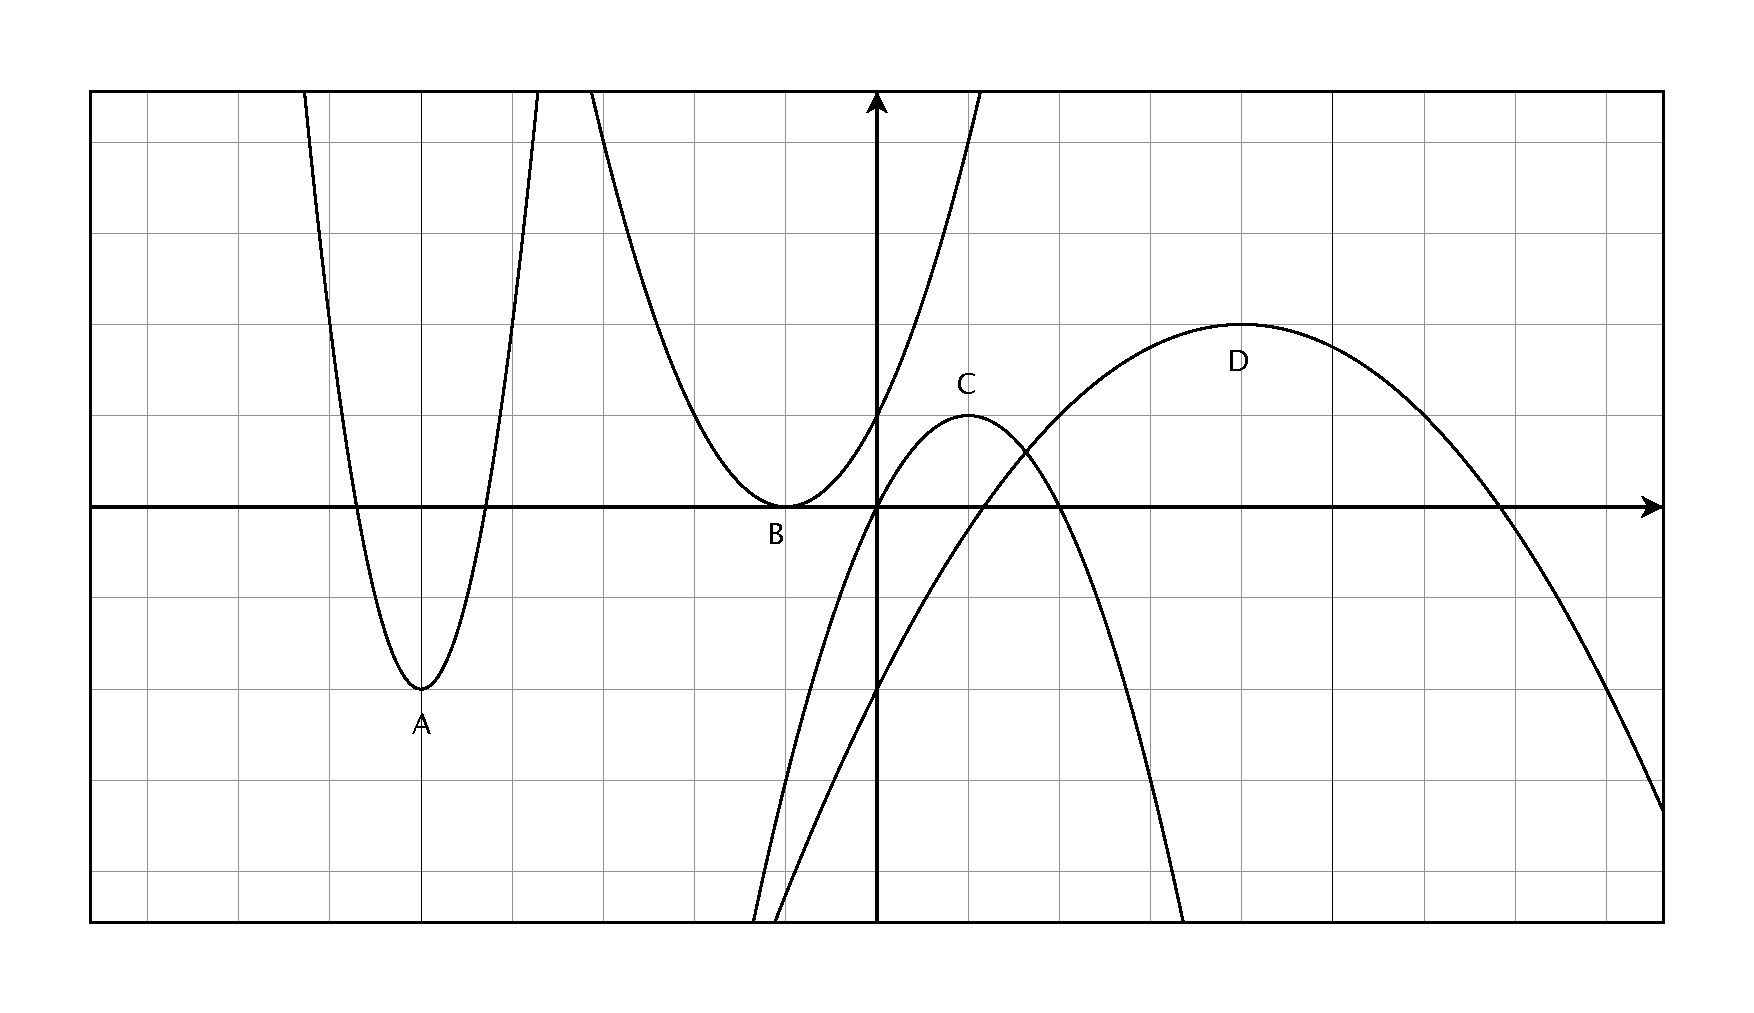
\includegraphics[scale=.3]{problem_7.eps}
%   \caption*{Problem 7}
% \end{figure}

% \begin{tabular}{cc}
% \toprule
% period & amplitude \\
% \midrule
%   $\pi$ & $2$ \\
% \bottomrule
% \end{tabular}

\title{Math 142 Notes \\ Section 5.3}

\date{September 11, 2013}

\begin{document}

  \maketitle
  \tableofcontents

  \section{Basic Graph}

  \begin{itemize*}
    \item draw single period of sine using known points
    \item draw single period of cosine using known points
  \end{itemize*}

  \begin{itemize*}
    \item sine, cosine, etc., repeat as you go around the unit circle again
    \item $\sin(t \pm 2n \pi) = \sin t$ for any integer $n$, etc.
    \item a function is periodic if there is some $p$ where $f(t + p) = f(t)$ for any value of $t$.  The smallest
      $p$ that works is the {\em period} of $f$.
    \item to graph a periodic function, you only need one period
    \item The period of sine and cosine is $2 \pi$.  
  \end{itemize*}

  \section{Amplitude}
  \subsection{Description}
  \[
    y = a \sin x
  \]

  \begin{itemize*}
    \item $|a|$ is the amplitude
    \item determines vertical scale
  \end{itemize*}

  \subsection{Examples}
  \begin{enumerate}
    \item $y = 2 \sin x$
    \item $y = \sfrac{1}{2} \sin x$
    \item $y = -3 \cos x$
  \end{enumerate}

  \section{Period}
  \[
    y = \sin kx
  \]

  \subsection{Shorter Period}
  $y = \sin 2x$

  \begin{tabular}[H]{lrr}
    $0$                & $0$                & $0$ \\
    $\sfrac{\pi}{4}$   & $\sfrac{\pi}{2}$   & $1$ \\
    $\sfrac{\pi}{2}$   & $\pi$              & $0$ \\
    $\sfrac{3 \pi}{4}$ & $\sfrac{3 \pi}{2}$ & $-1$ \\
    $\pi$              & $2 \pi$            & $0$ \\
  \end{tabular}

  Cycle repeats every $\pi$

  \subsection{Longer Period}
  $y = \sin \frac{1}{2} x$

  \begin{tabular}[H]{lrr}
    $0$     & $0$                & $0$ \\
    $\pi$   & $\sfrac{\pi}{2}$   & $1$ \\
    $2 \pi$ & $\pi$              & $0$ \\
    $3\pi$  & $\sfrac{3 \pi}{2}$ & $-1$ \\
    $4 \pi$ & $2 \pi$            & $0$ \\
  \end{tabular}

  Cycle repeats every $4 \pi$

  \subsection{General}
  \begin{align*}
    f(x)  & = \sin(x + 2 \pi n) \\
          & = \sin x \\
    \\
    f(kx) & = \sin(kx + 2 \pi n) \\
    f(kx) & = \sin(k (x + \frac{2 \pi}{k} n) \\
          & = \sin(kx) \\
  \end{align*}

  \begin{itemize*}
    \item $\sfrac{2 \pi}{k}$ is the period
    \item determines horizontal scale
    \item bigger $k$ means travel faster around the unit circle and a shorter period
    \item bigger $k$ means compressed horizontally
    \item $k = 1$ gives a period of $2 \pi$
  \end{itemize*}

  \subsection{Examples}
  \begin{enumerate*}
    \item $y = \sin 3x$; 
    \item $y = \sin \frac{3}{2} x$
  \end{enumerate*}

  \section{General Graph}
  \subsection{General Form}
  \[
    y = a \sin k(x - b)
  \]

  \begin{itemize*}
    \item $|a|$ is the amplitude---determines how big the peaks and valleys are
    \item $\frac{2 \pi}{k}$ is the period---determines the horizontal compression
    \item $b$ is the phase shift---determines the horizontal shift
    \item to graph one period, graph from $b$ to $b + \frac{2 \pi}{k}$
  \end{itemize*}

  \section{Examples}

  \begin{enumerate}
    \item $y = \sin x$
      \begin{align*}
        amplitude & = 1 \\
        period    & = 2 \pi \\
        phase     & = 0 \\
      \end{align*}

    \item $y = 2 \sin x$
    \item $y = - 2 \sin x$
  \end{enumerate}

\end{document}
